\subsection{Requirements} \label{ss:requirements}

\paragraph{Functional}
Using \projectname{}, employees (i.e., people who \gls{clock-in} and
\gls{clock-out}) should be able to:

\begin{itemize}
  \item Log into their account
  \item View assigned jobs
  \item View expected \& confirmed clock-ins \&
        clock-outs
  \item Verify attendance at jobs
\end{itemize}

In addition to the requirements for employees, managers
(i.e., people in charge of employees) should be able to:

\begin{itemize}
  \item View the verification chain for a job
\end{itemize}

\paragraph{Non-functional}
% TODO

In essence, the non-functional requirements are encompassed
by the \enquote{universal} guideline in the
\hyperref[s:motivation]{project motiviation}.

\subsection{Diagrams}

See Figures \ref{fig:erd}.

\begin{figure}[h]
  \centering
  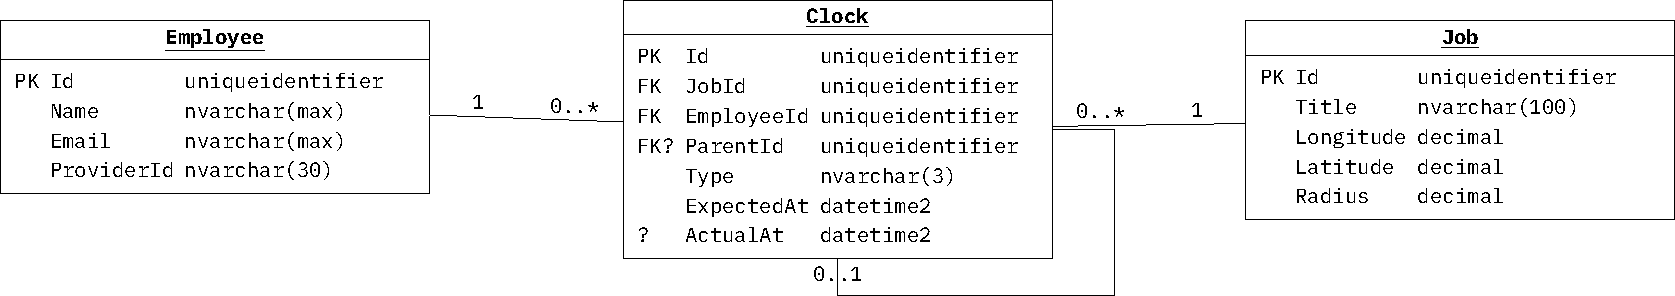
\includegraphics[width=\linewidth]{05 design/assets/entity relationship diagram.pdf}
  \caption{Entity Relationship Diagram}
  \label{fig:erd}
\end{figure}